\documentclass{report}
\usepackage[T1]{fontenc} % Fontes T1
\usepackage[utf8]{inputenc} % Input UTF8
\usepackage[backend=biber, style=ieee]{biblatex} % para usar bibliografia
\usepackage{csquotes}
\usepackage[portuguese]{babel} %Usar língua portuguesa
\usepackage{blindtext} % Gerar texto automaticamente
\usepackage[printonlyused]{acronym}
\usepackage{hyperref} % para autoref

\usepackage{}\usepackage{graphicx}

\bibliography{bibliografia}


\begin{document}
%%
% Definições
%
\def\titulo{Projeto Object Detection}
\def\data{16-05-2019}
\def\autores{João Gameiro , Pedro Pereira, Marco Ramos, Tiago Pedrosa}
\def\autorescontactos{(93097) joao.gameiro@ua.pt, (93196) pedrocjdpereira@ua.pt, (93388) msramos99@ua.pt, (93389) pedrosa.tiago@ua.pt}
\def\versao{VERSAO}
\def\departamento{LABI - DETI}
\def\empresa{Universidade de Aveiro}
\def\logotipo{ua.pdf}
%
%%%%%% CAPA %%%%%%
%
\begin{titlepage}

\begin{center}
%
\vspace*{50mm}
%
{\Huge \titulo}\\ 
%
\vspace{10mm}
%
{\Large \empresa}\\
%
\vspace{10mm}
%
{\LARGE \autores}\\ 
%
\vspace{30mm}
%
\begin{figure}[h]
\center
\includegraphics{\logotipo}
\end{figure}
%
\vspace{30mm}
\end{center}
%
\begin{flushright}
\versao
\end{flushright}
\end{titlepage}

%%  Página de Título %%
\title{%
{\Huge\textbf{\titulo}}\\
{\Large \departamento\\ \empresa}
}
%
\author{%
    \autores{}
}
%
\date{\data}
%
\maketitle{}

\pagenumbering{roman}

%%%%%% RESUMO %%%%%%

\begin{abstract}
Este documento serve como relatório para um projeto realizado no âmbito da disciplina de Laboratórios de Informática. O programa construído tem como objetivo tornar possível a visualização de uma biblioteca de imagens. Esta mesma biblioteca é utilizada por um programa que é capaz da procura e identificação de objetos em imagens.

Ao longo do relatório, é analisado e explicado o código do programa e do website que o acompanha, expondo todas as funções e características do projecto. Após isto, é efectuada uma demonstração do funcionamento do programa e do modo correto de interacção com a interface do mesmo e o relatório é concluído com algumas reflexões sobre o projeto e o contributo
que este teve para o desenvolvimento das nossas capacidades.


\end{abstract}
%%%%%% Agradecimentos %%%%%%
% Segundo glisc deveria aparecer após conclusão...


\tableofcontents
% \listoftables     % descomentar se necessário
% \listoffigures    % descomentar se necessário


%%%%%%%%%%%%%%%%%%%%%%%%%%%%%%%
\clearpage
\pagenumbering{arabic}

%%%%%%%%%%%%%%%%%%%%%%%%%%%%%%%%
\chapter{Introdução}
\label{chap.introducao}
O programa desenvolvido tem como objectivo permitir a visualização de uma biblioteca de imagens. Acompanhado de outra ferramenta, torna-se possível a procura e identificação de objetos das imagens armazenadas nessa mesma biblioteca.

O relatório está dividido em 5 capítulos. Depois deste \autoref{chap.introducao} (Introdução), encontra-se o \autoref{chap.desenvolve} (Desenvolvimento) onde é apresentado e explicado o código que foi desenvolvido. No \autoref{chap.result} (Resultados) é demonstrado o funcionamento do programa e no \autoref{chap.conclusao} apresentam-se as conclusões do projeto. Para acabar, é comentada a divisão do trabalho entre os elementos do grupo no \autoref{chap.div}.

\chapter{Desenvolvimento}
\label{chap.desenvolve}
\section{Python}

\subsection{Módulos}
Os módulos importados foram os seguintes:
\begin{itemize}
    \item Image : usado na manipulação e obtenção de informação de imagens;
    \item Sqlite3 : usado para operações relacionadas com a base de dados (incluindo criação e métodos);
    \item cherrypy : usado para o desenvolvimento da aplicação;
    \item json : funções de retorno de informação e para obtenção da mesma;
    \item requests : utilizado para a obtenção de informação do processador fornecido pelos docentes;
    \item hashlib : sintetização dos nomes das imagens;
    \item os.path : obtenção de informações sobre directórios.
\end{itemize}

O programa começa com a definição de um dicionário que contribui para a configuração da aplicação.


\subsection{Base de Dados}

Como podemos verificar na \autoref{fig:db} a criação da base de dados é feita sob a condição de que se não existir já uma é criada. São sintetizadas duas tabelas uma (Imagem) para guardar informações sobre a imagem original (id e nome original da mesma) e outra (Objecto) para guardar informações como: nome da imagem com o objecto extraído, nome do objecto, a cor do objecto, a confiança usada e o id da imagem original. 

\begin{figure}[h]
\center % Centra as imagens
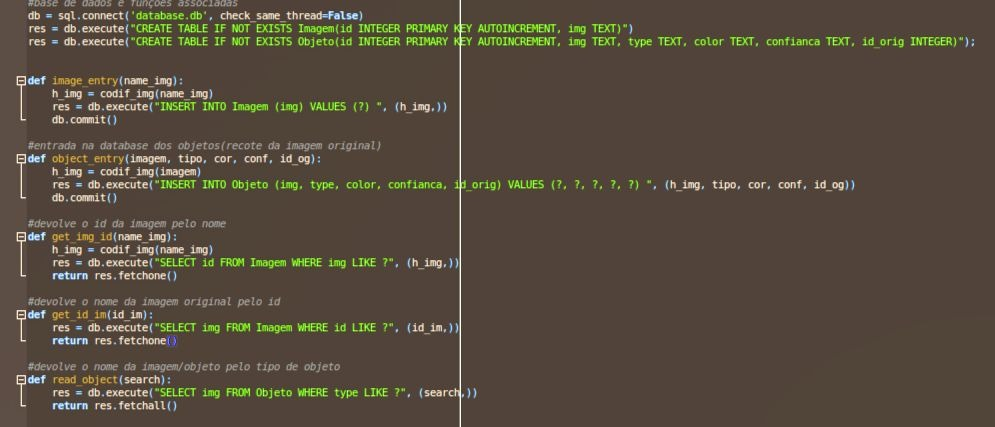
\includegraphics[height=180pt]{db0.jpg}
\caption{Criação da Base de Dados e alguns métodos}
\label{fig:db}
\end{figure}


Posteriormente à criação da base são definidos vários métodos com a sua função descrita na \autoref{table:dbm}


\begin{table}[h]
\centering
\caption{Métodos da Base de dados}
\begin{tabular}{r|lr}
 
Métodos & Função \\ 
\hline                               
\texttt{imag\_entry}& Inserir o nome da imagem na tabela Imagem \\
\texttt{objetc\_entry} & Inserir dados em todas as entradas da tabela Objeto  \\
\texttt{get\_im\_id} & Obter o id de uma imagem inserindo-se o nome da mesma \\
\texttt{get\_id\_im} & Oposto da anterior (obter nome inserindo-se o id) \\
\texttt{read\_object} & Devolve o nome da imagem pequena com o objeto extraído inserindo-se o objeto  \\
\texttt{read\_obj\_col} &  Devolve o nome da imagem pequena tendo em conta o tipo de objeto e cor inseridos\\
\texttt{return\_obj} & Devolve todos os objetos  
 
 \label{table:dbm}
\end{tabular}
\end{table}



\subsection{Funções Adicionais}
\subsubsection{\texttt{codif\_im}}

Esta função serve para sintetizar um nome "encriptado" de uma imagem inserida como argumento.
É neste caso que é usado o módulo hashlib.

\subsubsection{\texttt{belongs\_box} e  \texttt{object\_extraction}}

A função \texttt{object\_extraction} depende da primeira na medida em que é nestas duas que é realizado o processo de criação de uma nova imagem com o objeto extraído. A primeira verifica se um dado pixel pertence a uma certa área definida na informação que é fornecida pelo processador do docente. A segunda função analisa todos os píxeis de uma imagem e se estes pertencerem à área definida (usando a função anterior) então vão ser guardados numa nova imagem, caso contrário são descartados. 

\subsubsection{\texttt{color\_detetion}}
Esta última função serve para detectar a cor predominante numa imagem. Analisando a imagem usando o modo rgb, verifica-se a intensidade de cada um dos canais e dependendo do valor obtido irá dar retorno à cor predominante. Devido à dificuldade em estabelecer intervalos específicos para cada cor esta ferramenta não é totalmente confiável podendo devolver cores diferentes do esperado. 


\subsection{Interligação das Páginas e Listas}

Posteriormente passámos à interligação das páginas que constituíam a interface da aplicação. No entanto na \autoref{fig:Listas} aparece a definição de um conjunto de listas a anteceder a interligação das páginas. Essas listas serviram para auxiliar no armazenamento de informação e em comentário pode ser encontrada a definição seu conteúdo.

\begin{figure}[h]
\center % Centra as imagens
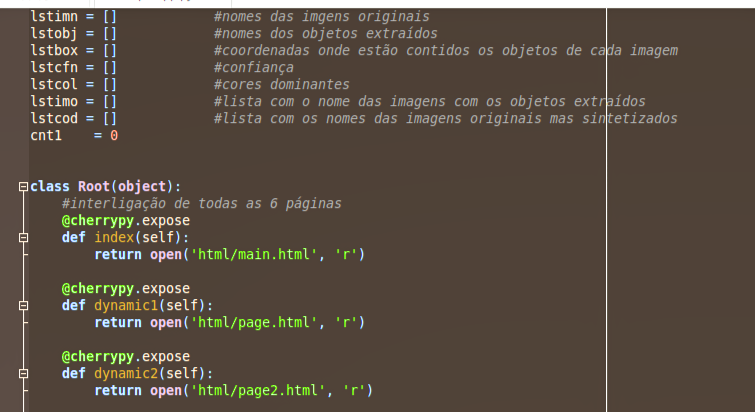
\includegraphics[height=180pt]{fd.png}
\caption{Interligação das Páginas e Listas}
\label{fig:Listas}
\end{figure}


\subsection{Função {\itshape list}}
Esta representa a função principal da aplicação sendo que é através da mesma que é recebida e tratada a informação para o sistema.

Através do expose da função {\itshape{put}} é enviada uma imagem para o sistema. Na função {\itshape list} a informação proveniente do processador é armazenada nas listas e na base de dados e posteriormente exposta ao cliente em diferentes locais da aplicação.

Na \autoref{fig:dbe} podemos visualizar a inserção da informação proveniente do processamento da imagem na base de dados (usando métodos já anteriormente descritos) e em listas para auxiliar no tratamento de informação e em revelação de erros e bugs.


\begin{figure}[h]
\center % Centra as imagens
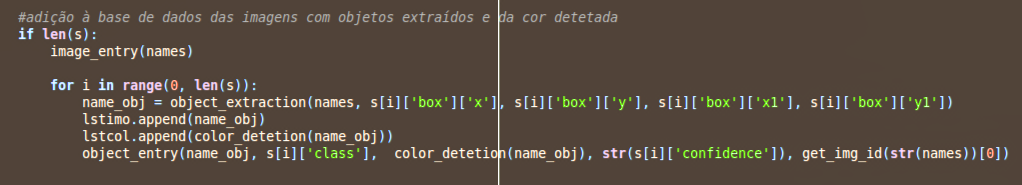
\includegraphics[height=70pt]{dbimage.png}
\caption{Inserção de informação na Base de Dados}
\label{fig:dbe}
\end{figure}


Na \autoref{fig:json} já podemos encontrar a devolução da informação obtida pelo processamento da imagem em forma de JSON ao cliente.Toda esta informação é apresentada ao carregar nos vários botões espalhados pela aplicação. 

Um dos casos de devolução é o nome dos objectos detectados até ao momento.

Os outros dois casos dependem de uma pesquisa efectuada pelo cliente, tendo num deles em conta apenas o tipo de objecto de detectado e noutro o tipo e a cor. Ou seja o cliente pesquisa pelo tipo de objecto e a aplicação devolve o nome das imagens (encriptado) com objectos já extraídos. O outro caso processa-se da mesma forma mas a pesquisa envolve também a cor.


\begin{figure}[h]
\center % Centra as imagens
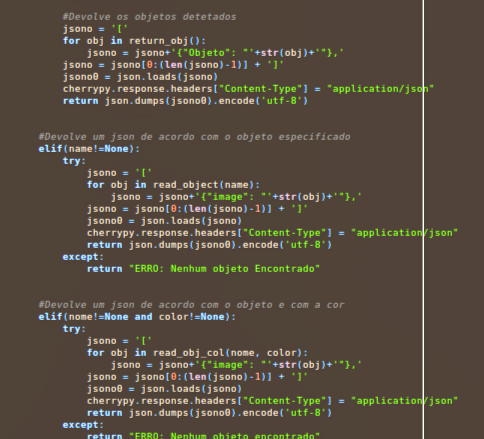
\includegraphics[height=250pt]{json.png}
\caption{Devolução de informação sob a forma JSON}
\label{fig:json}
\end{figure}


\subsection{Configuração e porta TCP}

Finalizando este capítulo temos na \autoref{fig:tcp} uma configuração da aplicação e da porta tcp usada.

\begin{figure}[h]
\center % Centra as imagens
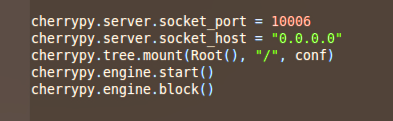
\includegraphics[height=90pt]{tcp.png}
\caption{Configuração e ligação ao servidor}
\label{fig:tcp}
\end{figure}



\section{HTML, CSS e JAVASCRIPT }

Na construção do website foi implementado uma barra de navegação no topo da página que permite acesso ao resto do conteúdo. Para além disto, foram costumizados o fundo e o tipo de letra e adicionado um rodapé para identificar os autores do trabalho. Todo o conteúdo utilizado na construção do website está disponibilizado nos urls seguintes.

\begin{itemize}
    \item Tipo de letra : http://fonts.googleapis.com/css?family=Ubuntu:bold e http://fonts.googleapis.com/css?family=Vollkorn
    \item Fundo do site : https://www.toptal.com/designers/subtlepatterns/
\end{itemize}

Concluindo este conteúdo não nos pertence apenas o usamos no desenvolvimento do estilo do nosso site e declaramos que o mesmo não é da nossa autoria.

O javacript usado serve para a inserção e apresentação de uma imagem na página html quando é inserida no sistema.
\chapter{Resultados}
\label{chap.result}

Na \autoref{fig:asp} podemos ver uma apresentação da página inicial da aplicação web desenvolvida, onde se pode observar a barra de tarefas que permite ligação entre páginas e um rodapé com os nomes dos autores.

\section{Aspecto Gráfico}
\begin{figure}[h]
\center % Centra as imagens
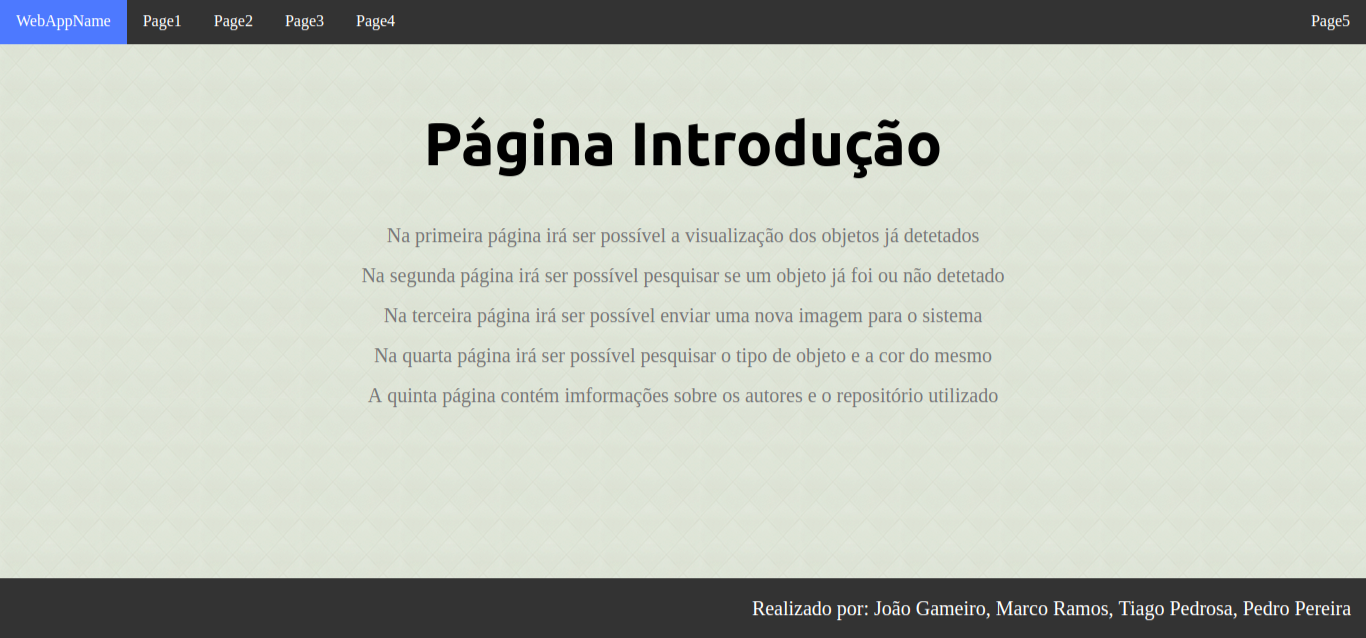
\includegraphics[height=150pt]{b.png}
\caption{Aspeto Gráfico da Aplicação e Teste Funcional}
\label{fig:asp}
\end{figure}


Se seleccionarmos a página 3 vamos obter à interface gráfica visível na \autoref{fig:se}. A partir desta página é possível enviar uma imagem nova, sendo para esse efeito apenas necessário carregar no botão "Choose File". Após isso a imagem será apresentada e seguidamente ao processamento da mesma vamos poder observar um JSON que identifica o objecto detectado. Na \autoref{fig:se} pode-se visualizar um exemplo que é uma imagem contendo um carro amarelo e o JSON devolvido pode ser visto na figura \autoref{fig:s}. Este JSON é nos devolvido numa nova página em branca com o único objectivo de devolver este pedaço de informação.

\begin{figure}[h]
\center % Centra as imagens
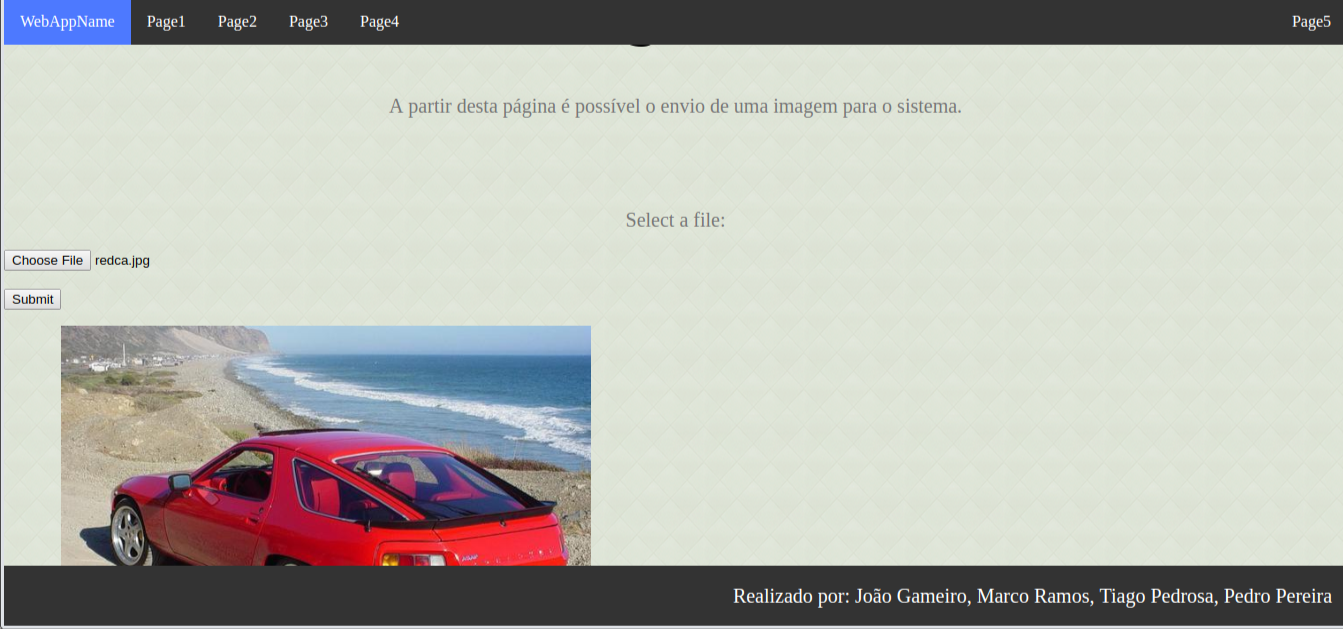
\includegraphics[height=120pt]{s.png}
\caption{Aspeto Gráfico da Página de envio de Imagem}
\label{fig:se}
\end{figure}


\begin{figure}[h]
\center % Centra as imagens
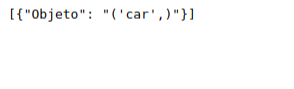
\includegraphics[height=120pt]{p.png}
\caption{JSON Devolvido}
\label{fig:s}
\end{figure}

Se formos ao directório da aplicação vamos poder comprovar que se encontra lá uma nova imagem criada a partir da anterior mas apenas com o carro (o objecto extraído, \autoref{fig:car}).

\begin{figure}[h]
\center % Centra as imagens
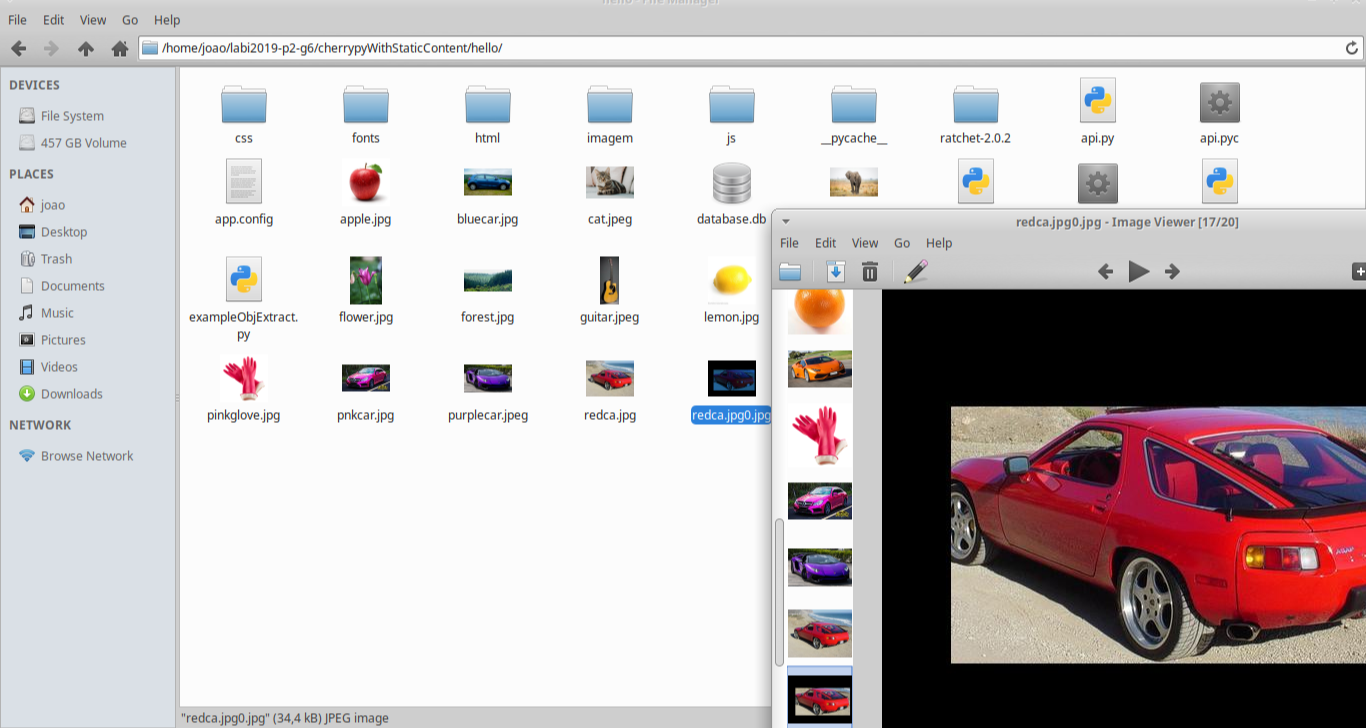
\includegraphics[height=130pt]{car.png}
\caption{Nova imagem criada apenas com o objeto}
\label{fig:car}
\end{figure}

Após verificar, testando as outras páginas, passando à pagina 1, vemos um botão que diz JSON. Ao carregarmos nele somos levados para uma nova página branca que devolve o objecto detectado, o nome da imagem original sintetizado, tal como o nome da nova imagem e a confiança usada (\autoref{fig:cef}).

\begin{figure}[h]
\center % Centra as imagens
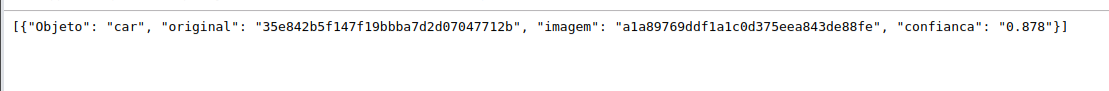
\includegraphics[height=30pt]{ggt.png}
\caption{JSON com o objeto, imagens  original e nova e confiança}
\label{fig:cef}
\end{figure}


Passando agora à página 2 em que se encontra uma barra de pesquisa. Insere-se o nome do objecto (neste caso "car") e somos direccionados para uma página em branca que possui um JSON com o nome da nova imagem sintetizado. \autoref{fig:as}.

Novamente mudando de página mas desta vez para a 4 encontramos duas barras de pesquisa, desta vez uma para o objecto e outra para a cor. Se inserirmos em cada barra "car" e "red" respectivamente vamos ser direccionados para outra página em branco que terá o mesmo conteúdo que a anterior visto que o sistema apenas tem uma imagem (um JSON com o nome da nova imagem sintetizada), \autoref{fig:as}). Ou seja esta página serve para pesquisar das imagens obtidas as que contém o objecto e cor designados pelo cliente.

\begin{figure}[h]
\center % Centra as imagens
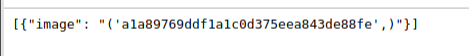
\includegraphics[height=30pt]{JSO.png}
\caption{Nome sintetizado de uma nova imagem}
\label{fig:as}
\end{figure}


Testando agora o detetor de cor. Enviando uma nova imagem, mas desta vez com um carro amarelo,verificamos se o sistema reconheceu ou não o objeto, e em caso afirmativo passamos para a página 4. Pesquisamos "car" e "yellow" (\autoref{fig:4}) e verificamos o resultado obtido.


\begin{figure}[h]
\center % Centra as imagens
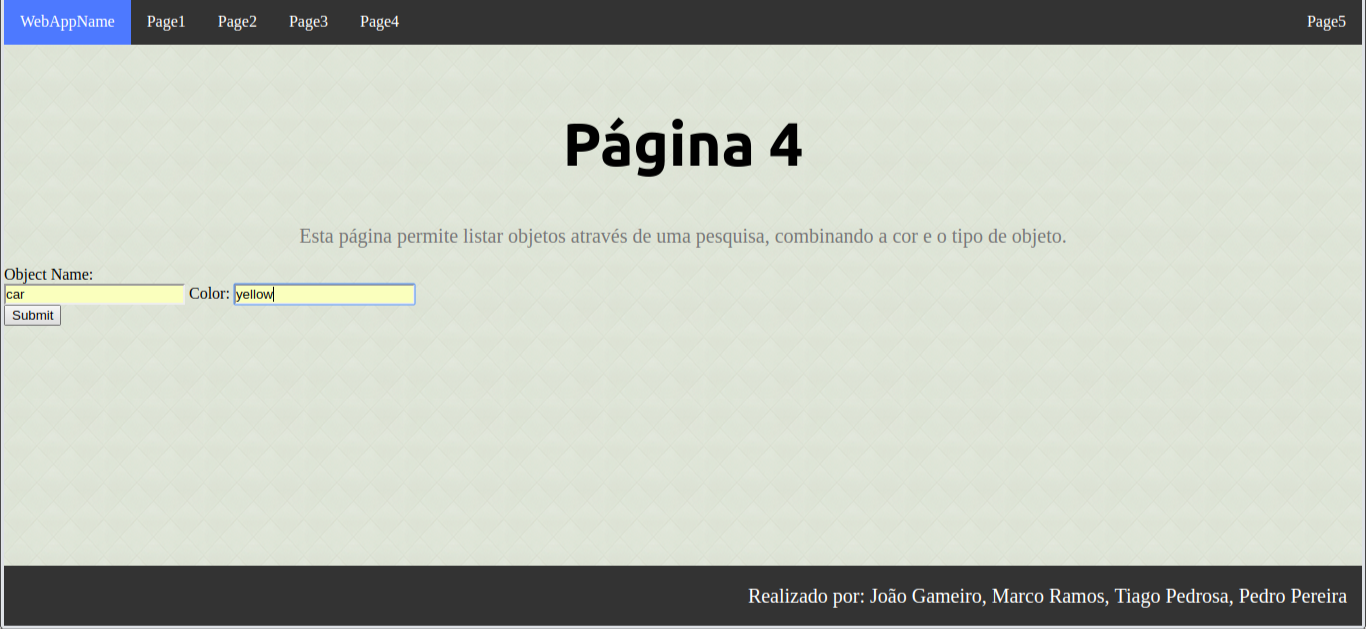
\includegraphics[height=170pt]{esta.png}
\caption{Interface da Página 4}
\label{fig:4}
\end{figure}


\begin{figure}[h]
\center % Centra as imagens
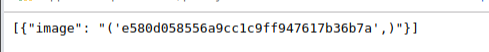
\includegraphics[height=40pt]{maisuma.png}
\caption{Resultado da Pesquisa yellow car}
\label{fig:carree}
\end{figure}

Como podemos comprovar a o nome sintetizado na \autoref{fig:carree} é diferente do sintetizado na \autoref{fig:as}, ou seja a aplicação devolveu a figura com o carro a amarelo e não a figura com o carro vermelho.




\section{Objetivos não cumpridos}

Listar objetos na página destinada a isso e apresentação de imagens nas páginas 2 e 4 e uma das funções que devolve JSON possui erros.  





\chapter{Conclusão}
\label{chap.conclusao}
 Não foi possível implementar todas as funcionalidades exigidas no enunciado, no entanto achamos que este projecto contribui bastante para a valorização do nosso percurso académico, tendo em conta que adquirimos competências nas áreas do desenvolvimento de aplicações web, manipulação de imagens e bases de dados. Reconhecemos também que contribuiu positivamente para a nossa capacidade de trabalhar em equipa, discussão, e aceitação de ideias provenientes de outros.
 
 Concluindo, sabemos que não atingimos todos os objectivos esperados neste projecto, mas concluímos que foi uma experiência que enriqueceu o nosso percurso académico, e reconhecemos também que trabalhámos arduamente para o que apresentamos aqui. 




\chapter{Divisão do trabalho entre os quatro elementos do grupo}
\label{chap.div}

A divisão do trabalho foi feita da seguinte forma:

\ac{jg} e \ac{mr} desenvolveram em conjunto o python e a base de dados presente neste projecto, discutindo, planeando e estruturando o código juntos.

\ac{pp} e \ac{tp} assumiram responsabilidade pelo design e aspecto gráfico da aplicação, tendo também ambos discutido e planeado a sua parte em conjunto.

É importante referir que apesar desta divisão todo o projecto foi discutido, planeado e estruturado pelos 4 membros e tal como descrito na aplicação concluímos que todos participaram igualmente neste projecto logo as percentagens representativas do trabalho de cada autor são:
 \begin{itemize}
     \item \ac{jg} - 25\%
     \item \ac{mr} - 25\%
     \item \ac{pp} - 25\%
     \item \ac{tp} - 25\%
 \end{itemize}
 
 O relatório foi escrito por \ac{pp} e por \ac{jg}.
 \ac{pp} escreveu o resumo, introdução e o capítulo sobre HTML e CSS. O conteúdo restante foi escrito por \ac{jg}.
 
 Foi usado um repositório na plataforma Code UA para o qual todos os autores contribuiu com commits frequentes. O link para esse repositório encontra-se na página 5 da aplicação desenvolvida.



%%%%%%%%%%%%%%%%%%%%%%%%%%%%%%%%%
\chapter*{Acrónimos}
\begin{acronym}
\acro{jg}[JG]{João Gameiro}
\acro{mr}[MR]{Marco Ramos}
\acro{pp}[PP]{Pedro Pereira}
\acro{tp}[TP]{Tiago Pedrosa}
\acro{ua}[UA]{Universidade de Aveiro}
\acro{miect}[MIECT]{Mestrado Integrado em Engenharia de Computadores e Telemática}
\acro{lei}[LEI]{Licenciatura em Engenharia Informática}

\end{acronym}


%%%%%%%%%%%%%%%%%%%%%%%%%%%%%%%%%
\printbibliography

\end{document}
\end{document}









